\section{Results}\label{sec:results}

\subsection{Employment in Selected Occupations}\label{sec:results:occupations}

Figure~\ref{fig:occupations_by_age} displays employment in four occupation groups with high theoretical AI exposure: software developers, ICT systems analysts, customer service agents, and ICT operations technicians.\footnote{ISCO-08 codes: software developers 2512--2514 and 2519; ICT systems analysts 2511; customer service agents 4222; ICT operations technicians 3511.} Each panel plots private-sector employment indexed to October 2022 = 1, separately by decade age group, with a vertical line marking the public release of ChatGPT on November 30, 2022.

In software development the 21--30 series falls to about 0.81 by early 2026, while the 31--40 and 51--60 series rise to roughly 1.16 and the 41--50 series is flat. ICT systems analysts and ICT operations technicians show the same shape, with the 21--30 series ending near 0.89 and 0.85. Customer service agents are noisier: the 21--30 series is roughly flat while the older groups end higher.

In all four occupations the youngest workers lose ground relative to older workers, the case-study pattern reported in \citet{brynjolfsson2025}. Section~\ref{sec:results:quintiles} incorporates all occupations systematically.

\begin{figure}[tp]
  \centering
  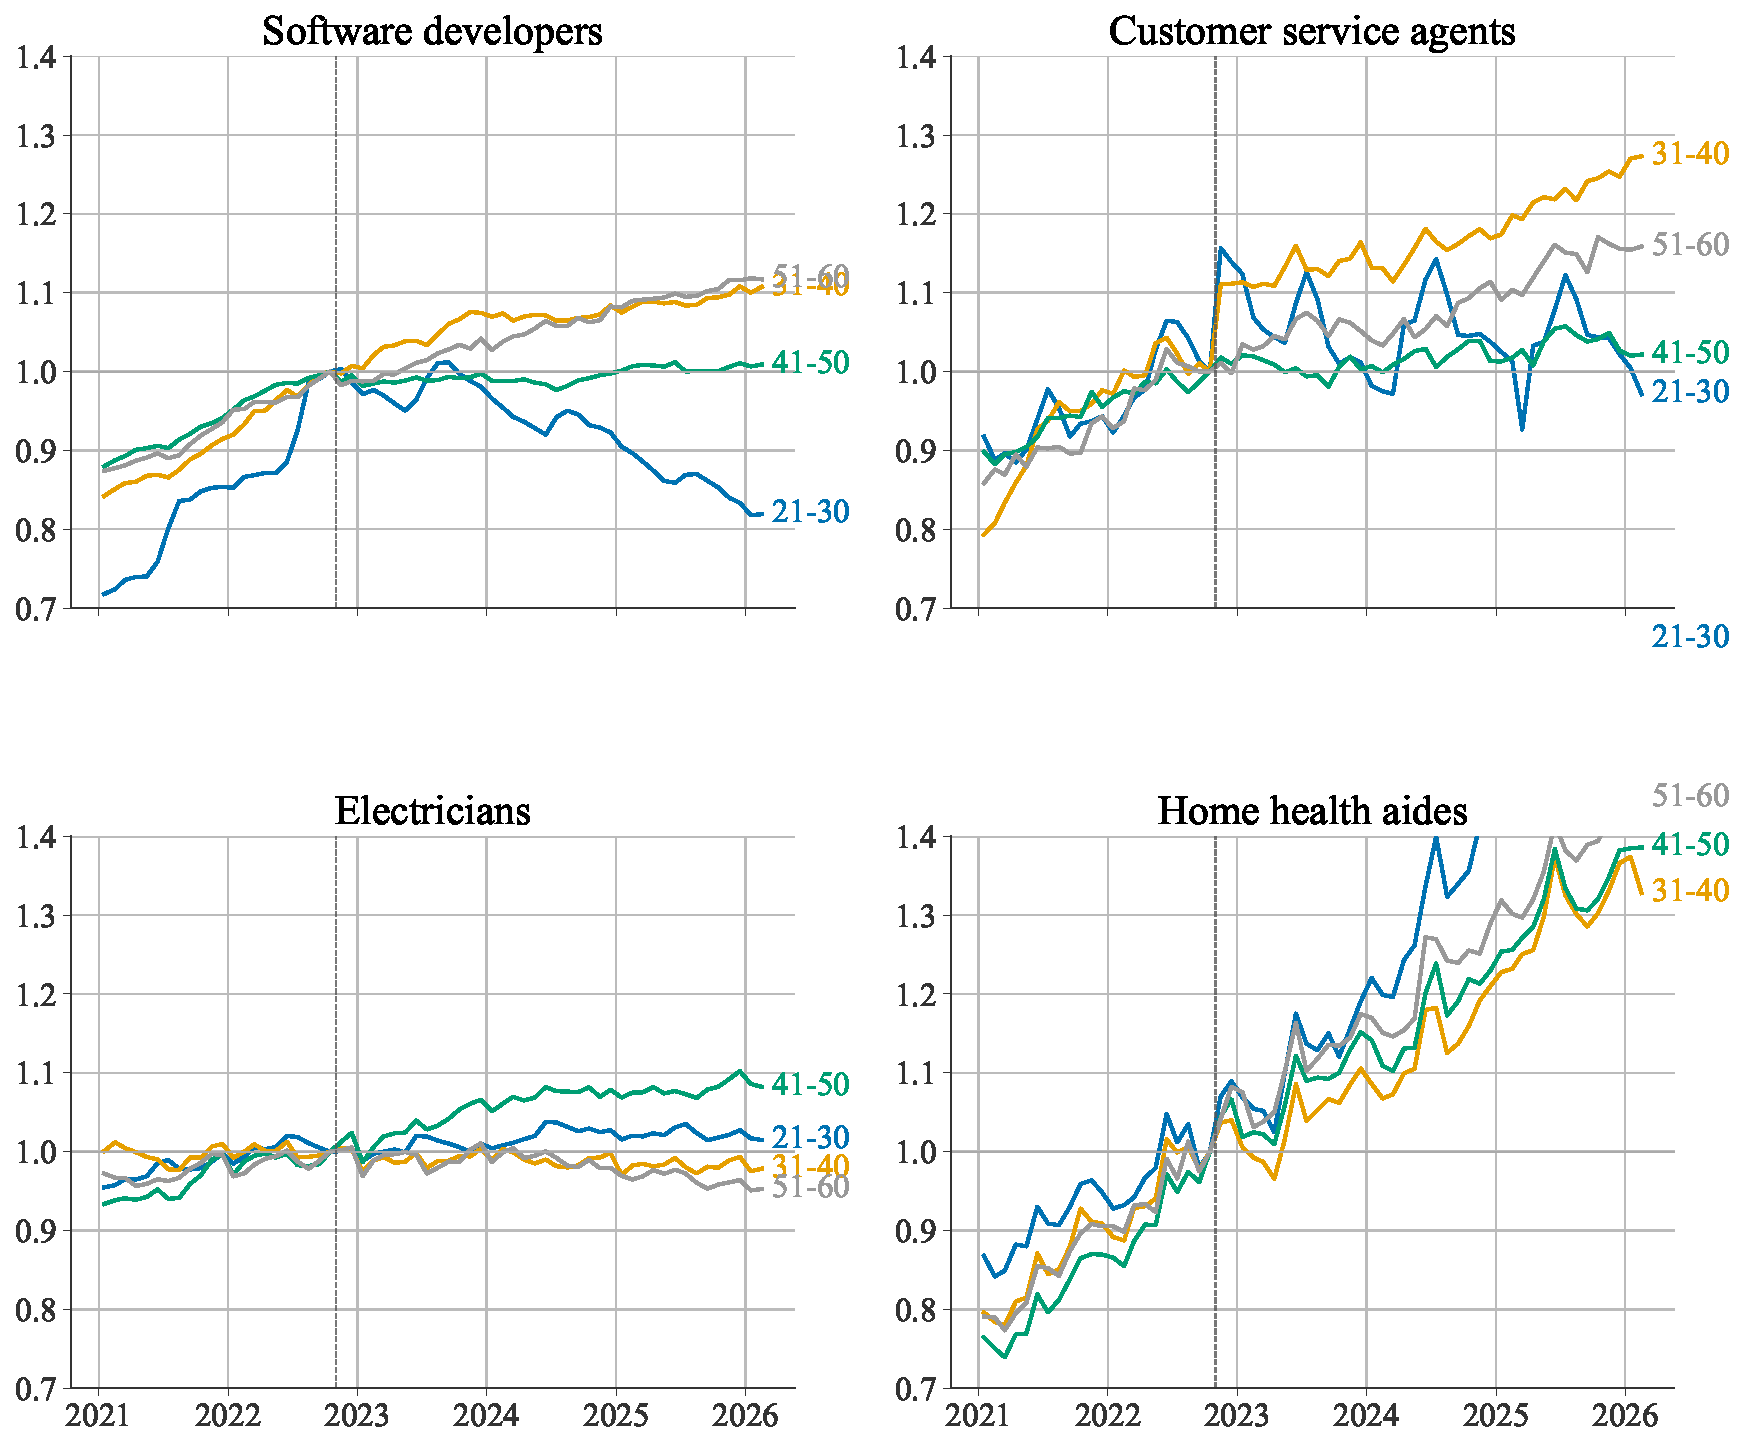
\includegraphics[width=\textwidth]{../analysis/output/figures/figure1_occupations_by_age.pdf}
  \caption{Employment in selected high-exposure occupations, by decade age group.}
  \label{fig:occupations_by_age}
  \begin{minipage}{\textwidth}\footnotesize\textit{Notes:} Private-sector employment per capita (headcount divided by resident population in the age group), indexed to October 2022 = 1. Panels show software developers (ISCO-08 2512--2514, 2519), ICT systems analysts (2511), customer service agents (4222), and ICT operations technicians (3511). The vertical dashed line marks November 30, 2022 (ChatGPT release).\end{minipage}
\end{figure}


\subsection{Employment by AI Exposure Quintile}\label{sec:results:quintiles}

The case studies above examine occupations chosen for their AI relevance. A more systematic approach ranks all occupations by their AI exposure score and examines whether high-exposure occupations exhibit different employment trends than low-exposure occupations. We assign each occupation to a quintile based on its Eloundou et al.\ GPT-4 exposure score, from Q1 (least exposed) to Q5 (most exposed), and plot normalized employment by quintile within each age group.

\subsubsection*{Eloundou et al.\ Exposure}

Figure~\ref{fig:age_by_quintile} plots quintile-by-age employment for the private sector, indexed to October 2022. Each of the four panels is one decade age group, with quintile lines running from light blue (Q1, least exposed) to dark blue (Q5, most exposed) and a red line for the overall age-group trend.

The most-exposed occupations do not lose ground among the youngest workers. In the 21--30 and 31--40 groups the Q5 series tracks or runs above Q1 after the ChatGPT release. The negative gradient appears instead at ages 41--50, where Q5 ends about four points below Q1 by early 2026. The 51--60 group shows no clear separation.

Table~\ref{tab:did_cell} reports the corresponding difference-in-differences estimates: the average post-October-2022 change in each quintile relative to Q1, by age group, for employment, new hires, and log monthly earnings. The employment estimates are positive and significant for the most-exposed quintiles at ages 21--40 (Q5 about $+0.07$ log points in both groups) and negative at 41--50 (Q5 $-0.053$, $p<0.05$). New hires fall for the most-exposed quintile at 41--50 (Q5 $-0.084$). Log earnings show no systematic exposure gradient.


\begin{figure}[tp]
  \centering
  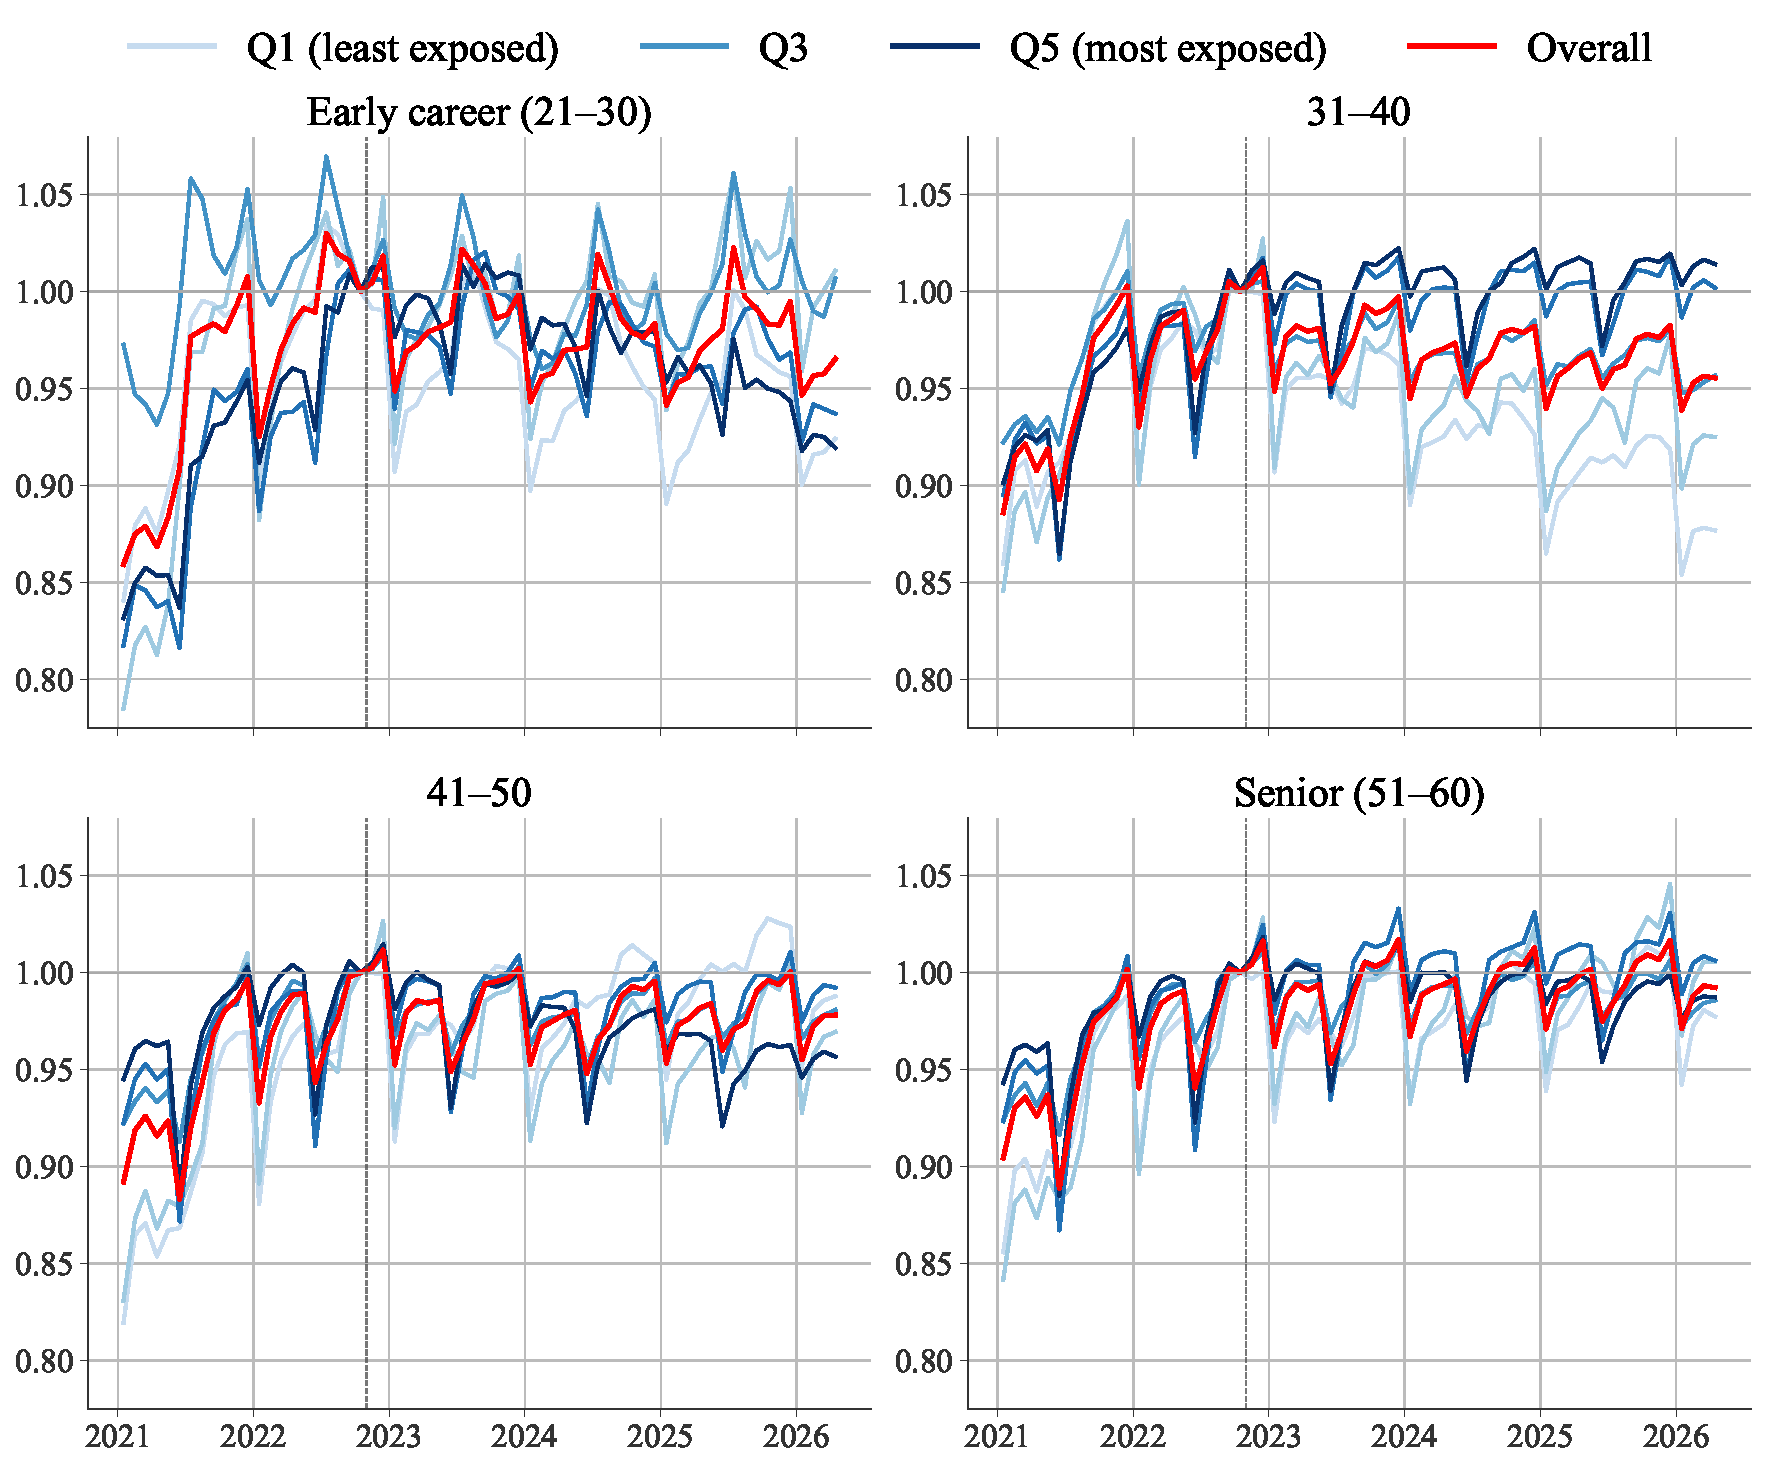
\includegraphics[width=\textwidth]{../analysis/output/figures/figure_emp_decade_private.pdf}
  \caption{Employment by AI-exposure quintile and decade age group, private sector.}
  \label{fig:age_by_quintile}
  \begin{minipage}{\textwidth}\footnotesize\textit{Notes:} Private-sector employment per capita (headcount divided by resident population in the age group), indexed to October 2022 = 1. Occupations are ranked by the Eloundou et al.\ GPT-4 exposure score. Q1 (lightest) = least exposed; Q5 (darkest) = most exposed. Red line = overall age-group trend. Vertical dashed line marks the November 2022 ChatGPT release.\end{minipage}
\end{figure}

\begin{table}[tp]
  \centering
  \caption{Cell-level difference-in-differences by AI-exposure quintile, private sector.}
  \label{tab:did_cell}
  \begin{tabular}{lcccc}
\toprule
 & Early career & 31--40 & 41--50 & Senior \\
 & (21--30) &  &  & (51--60) \\
 & (1) & (2) & (3) & (4) \\
\midrule
\multicolumn{5}{l}{\textit{Panel A. Employment (Poisson)}} \\
Q2 $\times$ Post & 0.0428 & 0.0181 & -0.0206 & 0.0080 \\
 & (0.0341) & (0.0357) & (0.0339) & (0.0268) \\
Q3 $\times$ Post & 0.0449$^{**}$ & 0.0432$^{***}$ & -0.0049 & 0.0102 \\
 & (0.0204) & (0.0167) & (0.0153) & (0.0135) \\
Q4 $\times$ Post & 0.0193 & 0.0707$^{***}$ & 0.0000 & 0.0216 \\
 & (0.0203) & (0.0169) & (0.0154) & (0.0134) \\
Q5 $\times$ Post & 0.0215 & 0.0783$^{***}$ & -0.0146 & 0.0103 \\
 & (0.0220) & (0.0186) & (0.0169) & (0.0166) \\
\addlinespace
\multicolumn{5}{l}{\textit{Panel B. New hires (Poisson)}} \\
Q2 $\times$ Post & 0.1247 & 0.2475$^{**}$ & 0.1836 & 0.2422$^{*}$ \\
 & (0.0810) & (0.1223) & (0.1247) & (0.1452) \\
Q3 $\times$ Post & 0.1158 & 0.1775$^{*}$ & 0.0999 & 0.0657 \\
 & (0.0740) & (0.1019) & (0.1100) & (0.1129) \\
Q4 $\times$ Post & 0.0713 & 0.1303 & 0.0591 & -0.0043 \\
 & (0.0770) & (0.1024) & (0.1074) & (0.1190) \\
Q5 $\times$ Post & -0.0424 & 0.0160 & -0.0116 & 0.0200 \\
 & (0.0845) & (0.1054) & (0.1104) & (0.1122) \\
\midrule
Occupations & 393 & 391 & 393 & 392 \\
Observations (count) & 24,366 & 24,242 & 24,366 & 24,304 \\
\bottomrule
\end{tabular}

  \begin{minipage}{\textwidth}\footnotesize\textit{Notes:} Each entry is the post-October-2022 change in the indicated quintile relative to Q1 (least exposed), by decade age group. Employment and new hires are Poisson; log monthly earnings is OLS weighted by cell employment. Occupation and month fixed effects; standard errors clustered by occupation. Sample 2021m1--2025m4. $^{*}$, $^{**}$, $^{***}$ denote $p<0.1$, $0.05$, $0.01$.\end{minipage}
\end{table}

The companion automation and augmentation quintile plots based on the Handa et al.\ decomposition are reported in Appendix Figures~\ref{fig:age_by_quintile_handa_auto} and~\ref{fig:age_by_quintile_handa_aug}.


\subsection{Automation versus Augmentation}\label{sec:results:auto_aug}

We follow \citet{brynjolfsson2025} on the automation-vs-augmentation split. Ranking the youngest workers by Handa automation share gives a modest negative gradient (Appendix Figure~\ref{fig:age_by_quintile_handa_auto}); ranking them by augmentation share gives no gradient at all (Appendix Figure~\ref{fig:age_by_quintile_handa_aug}). The split points toward displacement rather than augmentation, but the Handa classification only captures conversation mode, not what workers actually do on the job. An occupation scored as ``automation-exposed'' through conversation mode may in practice use AI for augmentation.


\subsection{Sector Heterogeneity}\label{sec:results:sectors}

The exposure gradient documented in Figure~\ref{fig:age_by_quintile} is a private-sector pattern. The public sector shows no exposure gradient in any age group (Appendix Figure~\ref{fig:emp_public}).

The public-sector null could reflect slower adoption, hiring insulated from market conditions, stronger employment protection, or a different occupational mix; we cannot separate these from the aggregate data. The adoption channel does have some support: \citet{riksrevisjonen2024} report that more than half of Norwegian state agencies have no experience with AI tools, so theoretical exposure in the public sector does not translate into implementation. The public sector is dominated by health, education, and administration; private high-exposure occupations cluster in IT, finance, and business services. 



\subsection{Wages and Other Outcomes}\label{sec:results:wages}

Figure~\ref{fig:kontantlonn_by_quintile} displays monthly cash earnings by Eloundou et al.\ exposure quintile and age group. Strong seasonal patterns dominate the wage plots: December earnings spike to 1.4--1.5 times the baseline due to Christmas bonuses, and June earnings are elevated due to statutory holiday pay. \citet{brynjolfsson2025} and \citet{humlum2026} find no wage divergence over a similar horizon in the US and Denmark. Norway's two-tier bargaining system \citep{bhuller2022} with sectoral wage floors and strong employment protection make the quantity margin the more likely site of adjustment.

Four additional outcomes are reported in the appendix: hourly wages (Figure~\ref{fig:timelonn_by_quintile}), contracted position percentage (Figure~\ref{fig:stillingspst_by_quintile}), overtime hours (Figure~\ref{fig:overtid_by_quintile}), and the share of new jobs (Figure~\ref{fig:nyjobb_by_quintile}). None shows a differential trend by exposure quintile, consistent with the extensive margin as the candidate site of adjustment.

\begin{figure}[tp]
  \centering
  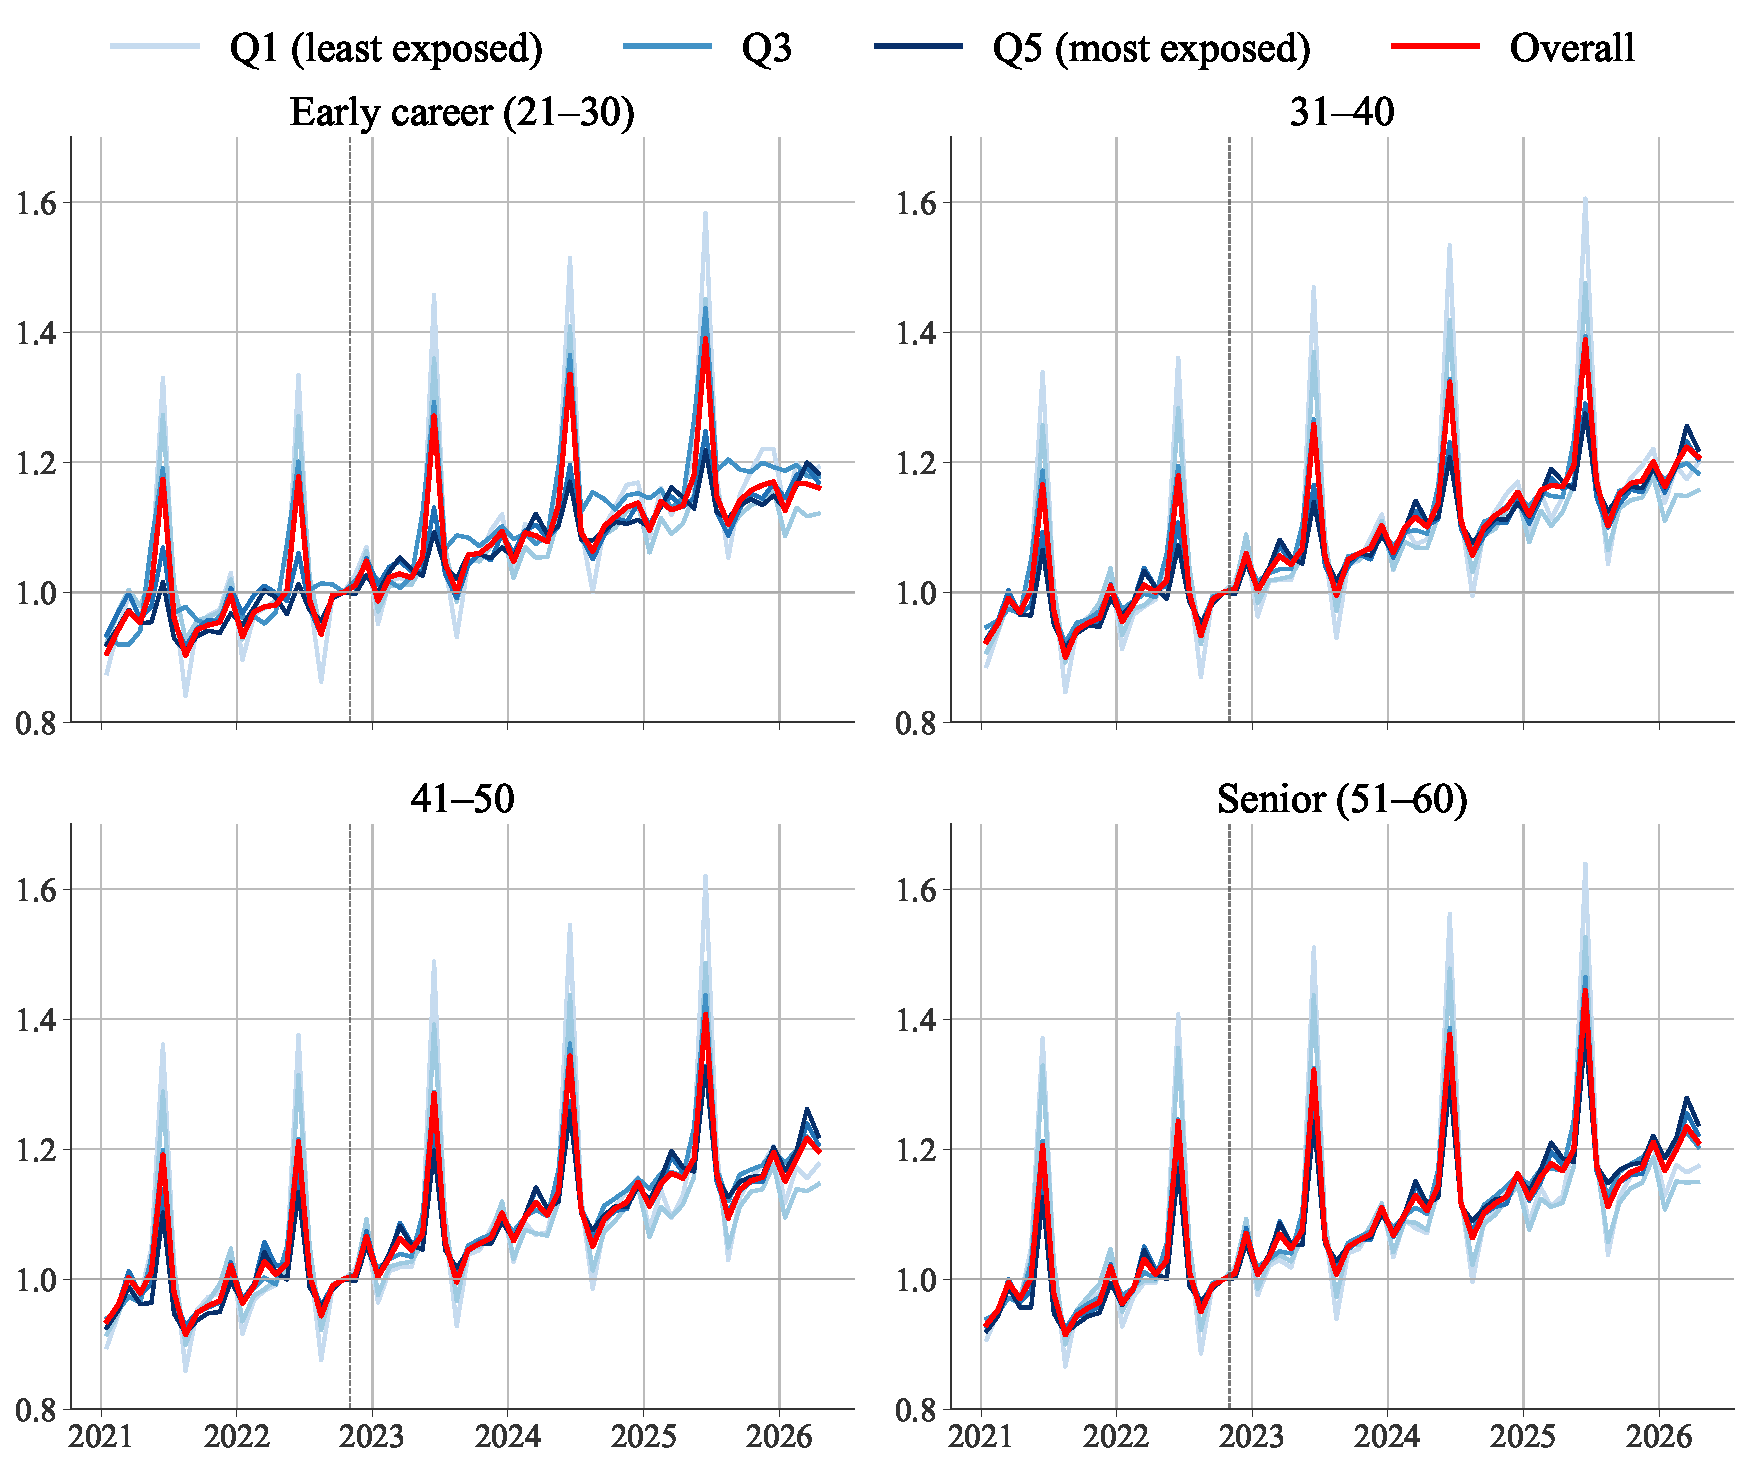
\includegraphics[width=\textwidth]{../analysis/output/figures/figure_kontantlonn_decade_private.pdf}
  \caption{Monthly cash earnings by AI-exposure quintile and decade age group, private sector.}
  \label{fig:kontantlonn_by_quintile}
  \begin{minipage}{\textwidth}\footnotesize\textit{Notes:} Mean monthly cash earnings, indexed to October 2022 = 1. Occupations are ranked by the Eloundou et al.\ exposure score. Strong seasonal patterns (December bonuses, June holiday pay) are visible in all panels.\end{minipage}
\end{figure}


\subsection{Poisson Regression Estimates}\label{sec:results:firmfe}

The quintile series so far normalize employment by the population in each age group, the right denominator for asking whether cohort-level employment shifts away from AI-exposed occupations. We turn now to the worker counts and ask if they reallocate across occupations? Following \citet{brynjolfsson2025}, we estimate Poisson event studies on the counts.

The cell-level microdata are tabulated at the (occupation $\times$ age group $\times$ month) level. We estimate
\[
\log E[\text{count}_{j,a,t}] = \alpha_{j} + \beta_{t} + \gamma_{q,k},
\]
separately per decade age group~$a$ in the private sector, where $j$ indexes occupations and $q(j)$ is the Eloundou GPT-4 $\beta$ quintile of occupation~$j$. The occupation FE absorbs the permanent employment level of each occupation; the month FE absorbs the aggregate time path of the age cohort. Standard errors are clustered at occupation. Reference: Q1 and $k=-1$ (October 2022).

Figure~\ref{fig:microdata_poisson_grid} reports the resulting $\gamma_{q,k}$ for $q\in\{2,3,4,5\}$ across the four decade age groups, in log points. The path matches the indexed series in Figure~\ref{fig:age_by_quintile}. At 41--50 the Q5 path turns negative after October 2022 and reaches about $-0.03$ log points by early 2026. At 21--30 the Q5 path is noisy and ends slightly positive; at 31--40 it rises to about $+0.11$; at 51--60 it stays near zero.

\begin{figure}[tp]
  \centering
  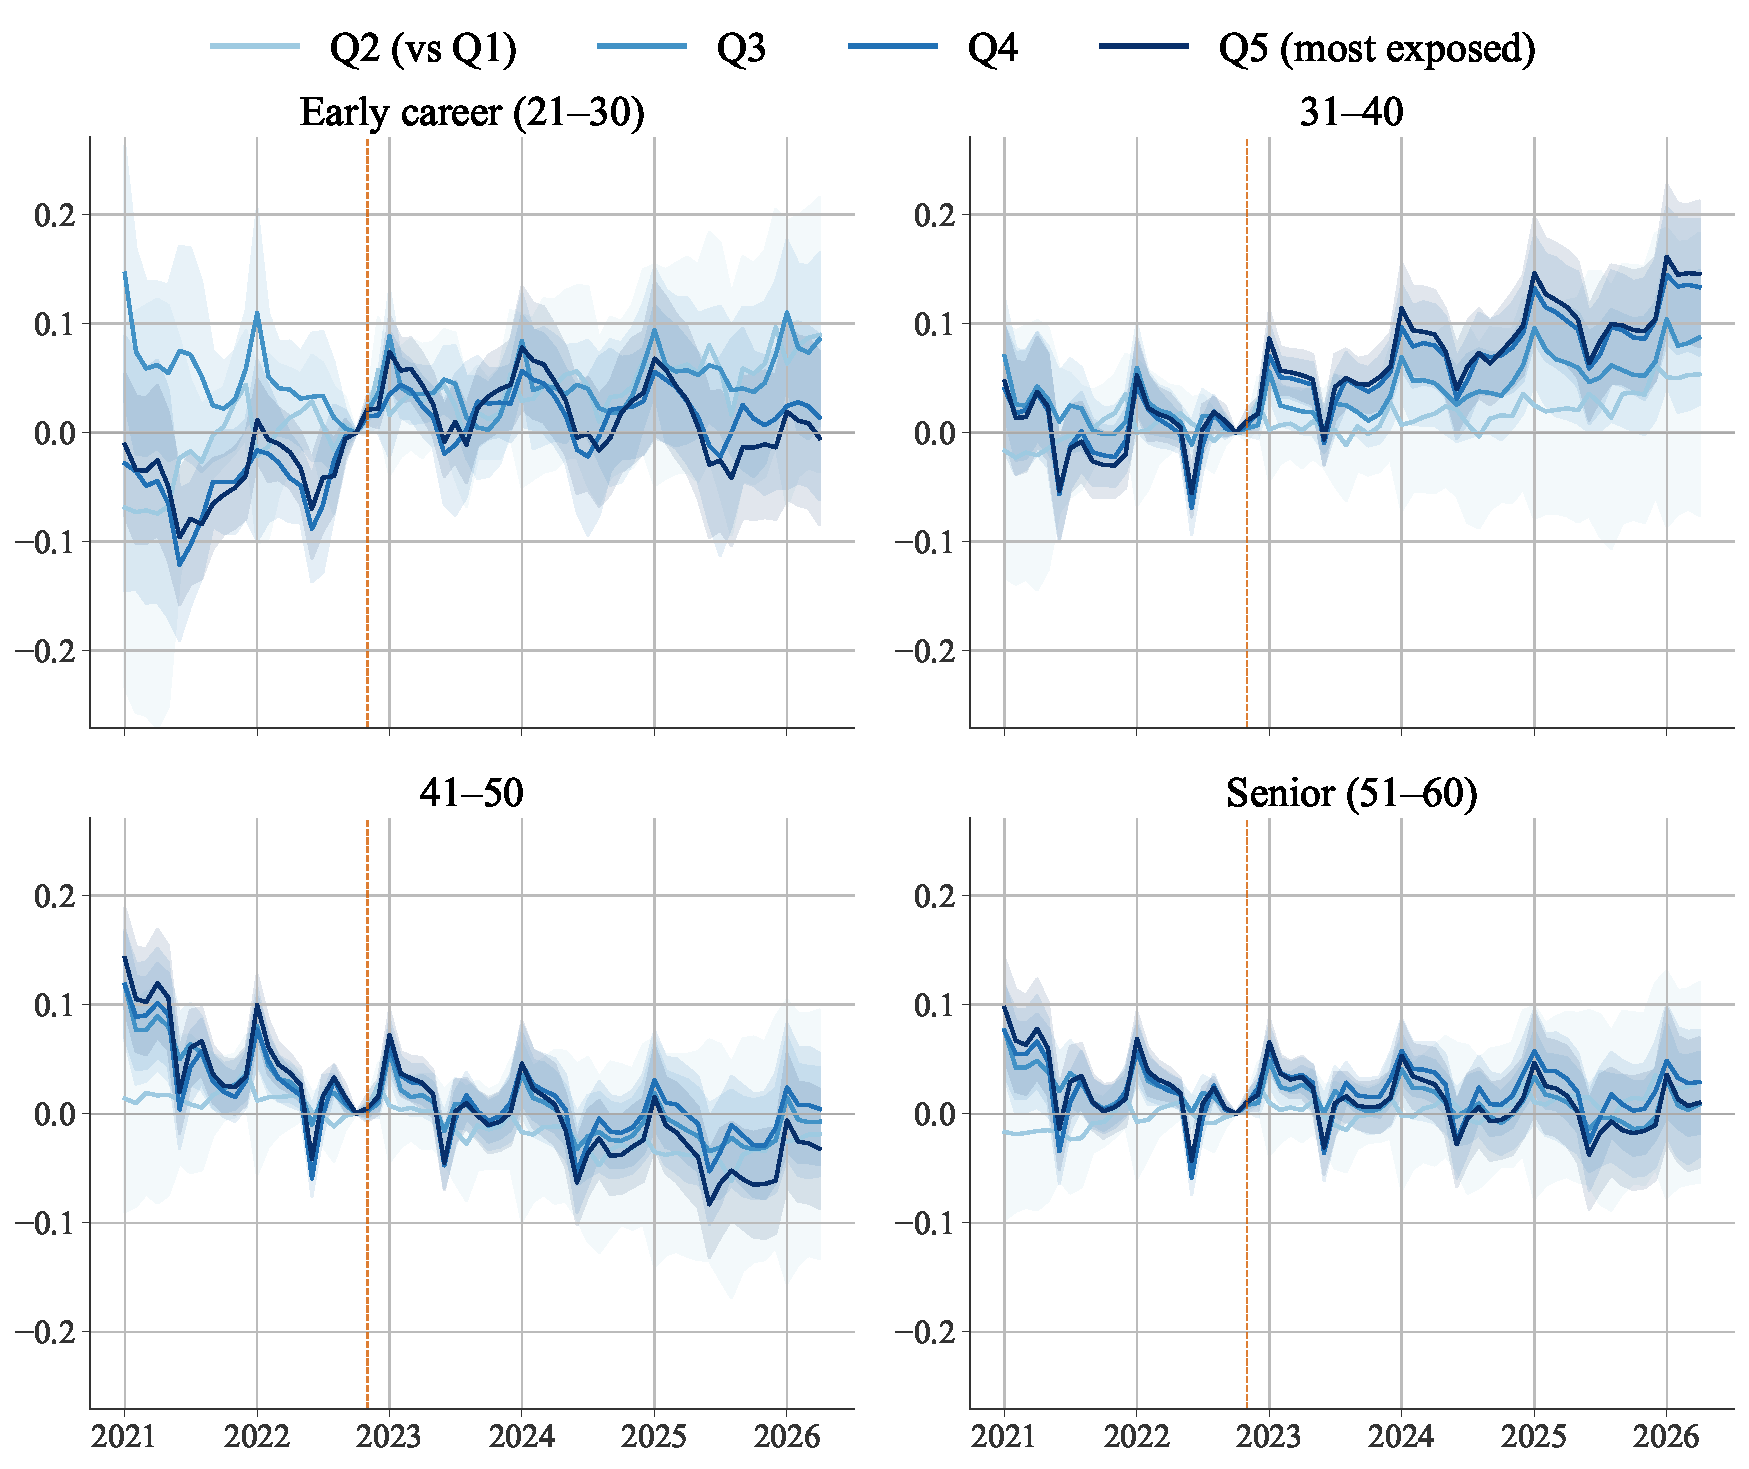
\includegraphics[width=\textwidth]{../analysis/output/figures/figure_microdata_poisson_es_grid.pdf}
  \caption{Poisson event-study coefficients by AI-exposure quintile and decade age group, private sector.}
  \begin{minipage}{\textwidth}\footnotesize\textit{Notes:} Coefficients $\gamma_{q,k}$ for $q\in\{2,\dots,5\}$ relative to $q=1$, in log points. Cell-level microdata.no aggregates (occupation\,$\times$\,age\,$\times$\,month), private sector; fixed effects for occupation and month. Sample 2021m1--2025m4. Shaded bands: 95\% confidence intervals clustered at occupation. Reference: October 2022. Dashed line marks the November 2022 ChatGPT release.\end{minipage}
  \label{fig:microdata_poisson_grid}
\end{figure}

The cell-level estimates absorb the average employment path of each occupation but do not separate reallocation \emph{within} firms from changes in the firm composition. Using the individual-level records on Statistics Norway's secure server, we estimate the within-firm composition design of \citet{brynjolfsson2025},
\[
\log E[\text{count}_{f,q,a,t}] = \alpha_{f,q} + \beta_{f,t} + \gamma_{q,k},
\]
on the panel of firm $f$ $\times$ quintile $q$ $\times$ month $t$ cells, separately per decade age group. Firm-by-quintile and firm-by-month fixed effects absorb the firm's persistent composition and any firm-level demand shock; identification rests on within-firm reallocation across exposure quintiles. Standard errors are clustered at the firm. The sample is private-sector \emph{foretak} with at least 20 workers in the 22--55 age window per month, January 2021 through July 2025 (the secure-server window is shorter than the cell-level data by seven months).

Figure~\ref{fig:firmfe_poisson_grid} reports the firm-FE $\gamma_{q,k}$. The qualitative pattern lines up with the cell-level estimates: at 41--50 the Q5 path drifts negative after late 2022, reaching about $-0.05$ log points by mid-2025; at 31--40 it rises to about $+0.10$; at 21--30 it is noisy with a sharp upward swing at the end of the window; at 51--60 it stays near zero. The within-firm comparison therefore does not reverse the cell-level pattern, suggesting that the post-2022 reallocation we document operates inside firms rather than only across them.

\begin{figure}[tp]
  \centering
  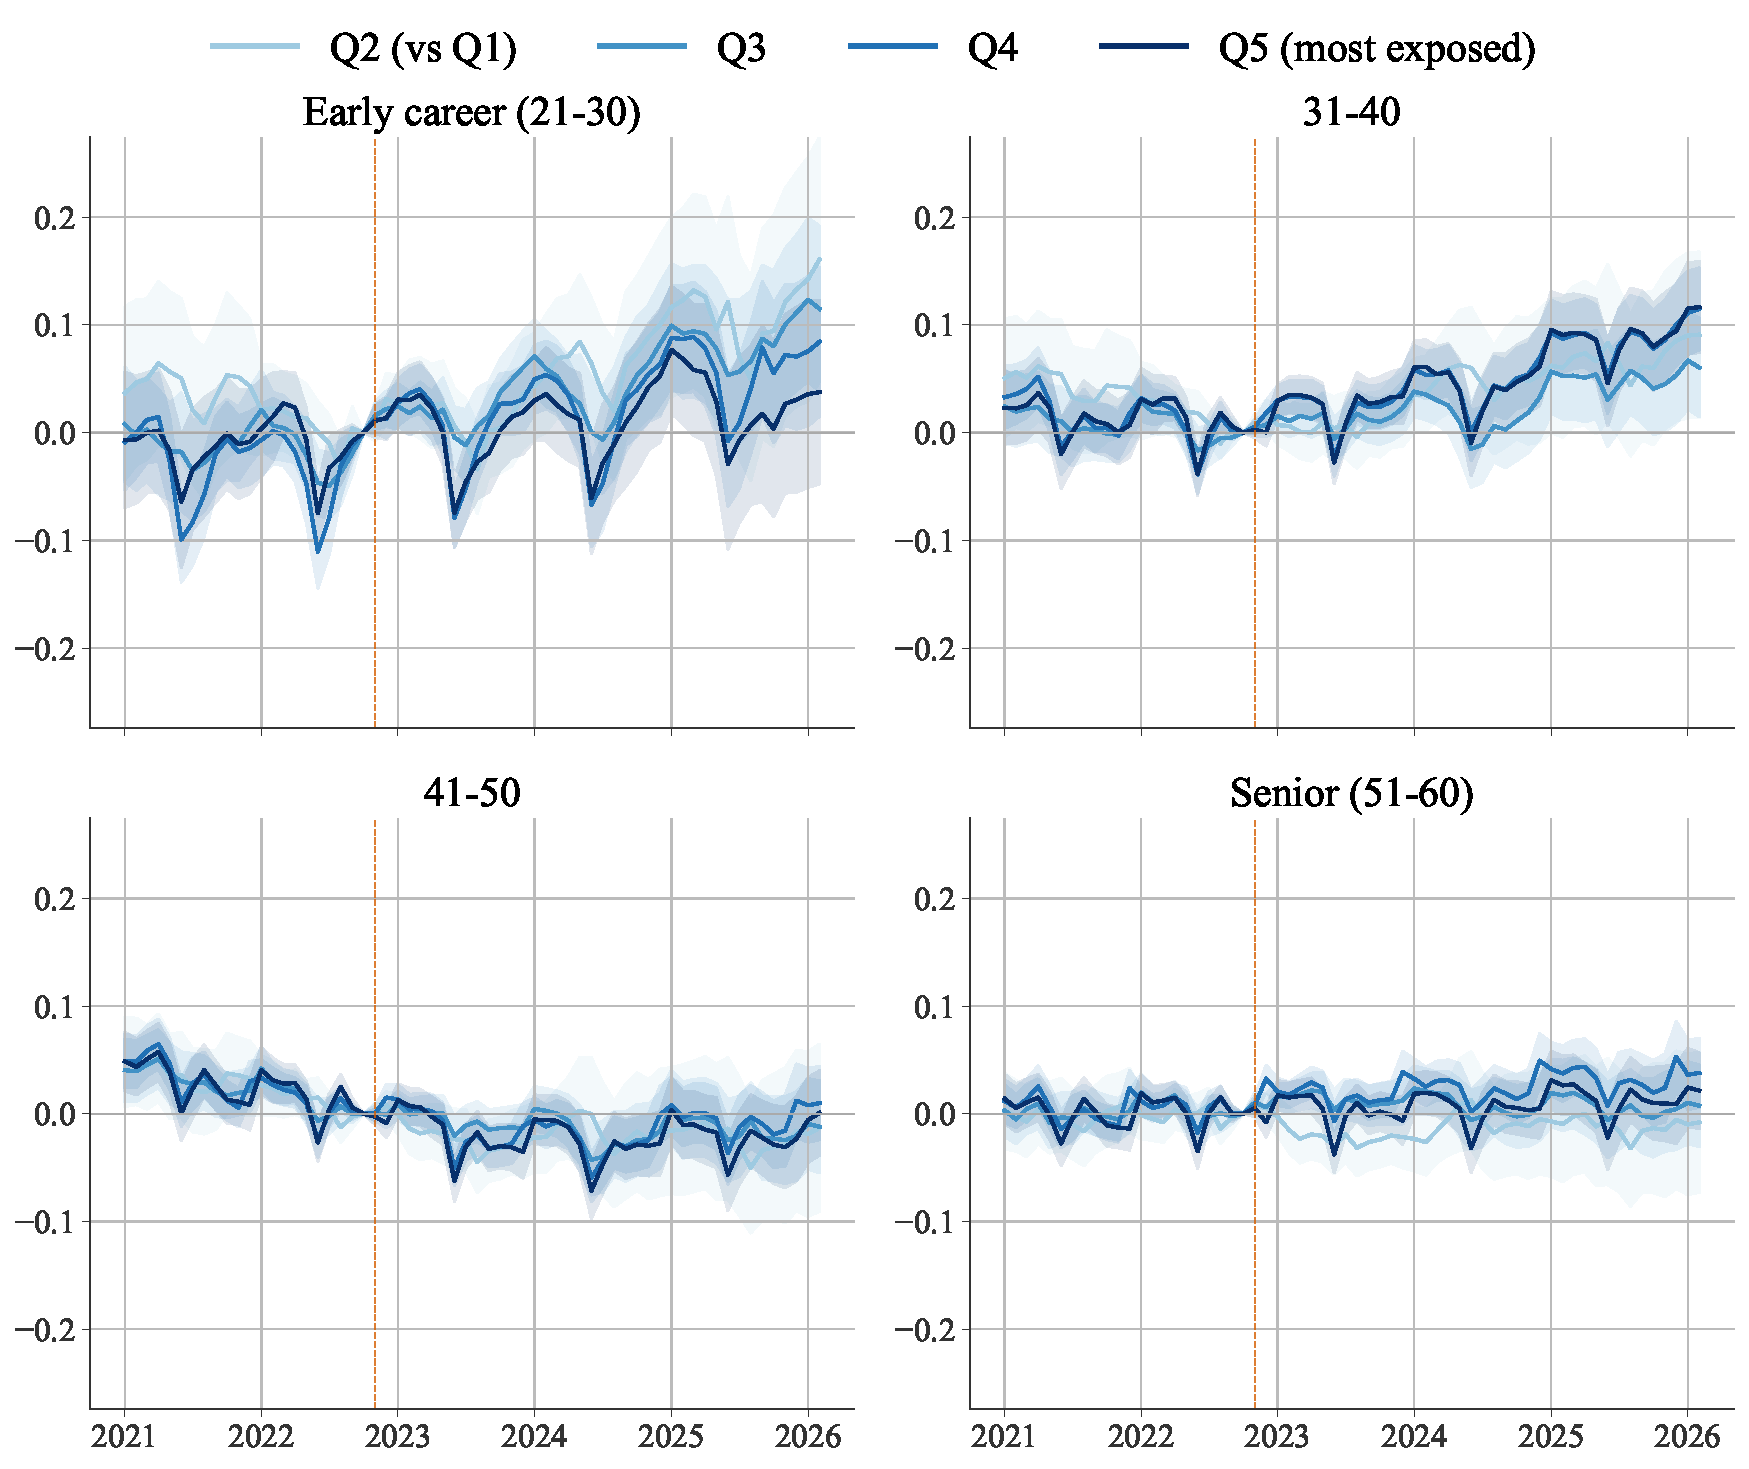
\includegraphics[width=\textwidth]{../analysis/output/figures/figure_firmfe_poisson_es_grid.pdf}
  \caption{Firm-fixed-effects Poisson event-study coefficients by AI-exposure quintile and decade age group, private sector.}
  \begin{minipage}{\textwidth}\footnotesize\textit{Notes:} Coefficients $\gamma_{q,k}$ for $q\in\{2,\dots,5\}$ relative to $q=1$, in log points. Estimated on the individual-level firm $\times$ quintile $\times$ month panel; fixed effects for firm $\times$ quintile and firm $\times$ month. Private-sector foretak with at least 20 workers in the 22--55 age window per month. Sample 2021m1--2025m7. Shaded bands: 95\% confidence intervals clustered at the firm. Reference: October 2022. Dashed line marks the November 2022 ChatGPT release.\end{minipage}
  \label{fig:firmfe_poisson_grid}
\end{figure}
